\documentclass[tikz,border=4pt]{standalone}
\usepackage{fontspec}\usepackage{xcolor}\usetikzlibrary{arrows.meta}
\setsansfont{Lato}
\definecolor{accent}{HTML}{1A3F6E}
\begin{document}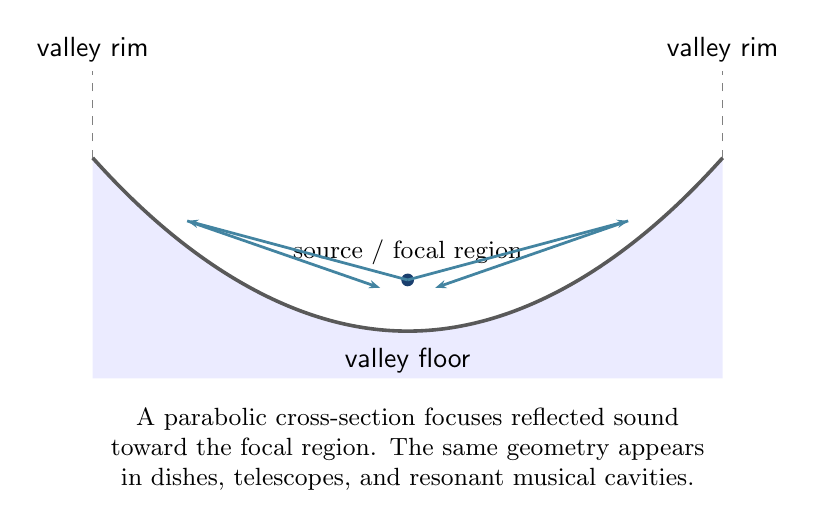
\begin{tikzpicture}[font=\sffamily]
\fill[blue!8] (-4,0) parabola bend (0,-2.2) (4,0) -- (4,-2.8) -- (-4,-2.8) -- cycle;
\draw[line width=1.3pt,gray!70!black] (-4,0) parabola bend (0,-2.2) (4,0);
\draw[dashed,gray] (-4,0) -- (-4,1.1); \draw[dashed,gray] (4,0) -- (4,1.1);
\node[above] at (-4,1.1) {valley rim}; \node[above] at (4,1.1) {valley rim};
\node[below] at (0,-2.3) {valley floor};
\fill[accent] (0,-1.55) circle (2.3pt); \node[above=2pt,font=\small] at (0,-1.55) {source / focal region};
\draw[-{Stealth[length=4pt]},cyan!60!black,line width=1pt] (0,-1.55) -- (-2.8,-.8);
\draw[-{Stealth[length=4pt]},cyan!60!black,line width=1pt] (0,-1.55) -- (2.8,-.8);
\draw[-{Stealth[length=4pt]},cyan!60!black,line width=1pt] (-2.8,-.8) -- (-.35,-1.65);
\draw[-{Stealth[length=4pt]},cyan!60!black,line width=1pt] (2.8,-.8) -- (.35,-1.65);
\node[text width=8cm,align=center,font=\small] at (0,-3.7) {A parabolic cross-section focuses reflected sound toward the focal region. The same geometry appears in dishes, telescopes, and resonant musical cavities.};
\end{tikzpicture}\end{document}
